\documentclass[11pt]{beamer}\usepackage[]{graphicx}\usepackage[]{xcolor}
% maxwidth is the original width if it is less than linewidth
% otherwise use linewidth (to make sure the graphics do not exceed the margin)
\makeatletter
\def\maxwidth{ %
  \ifdim\Gin@nat@width>\linewidth
    \linewidth
  \else
    \Gin@nat@width
  \fi
}
\makeatother

\definecolor{fgcolor}{rgb}{0.345, 0.345, 0.345}
\newcommand{\hlnum}[1]{\textcolor[rgb]{0.686,0.059,0.569}{#1}}%
\newcommand{\hlstr}[1]{\textcolor[rgb]{0.192,0.494,0.8}{#1}}%
\newcommand{\hlcom}[1]{\textcolor[rgb]{0.678,0.584,0.686}{\textit{#1}}}%
\newcommand{\hlopt}[1]{\textcolor[rgb]{0,0,0}{#1}}%
\newcommand{\hlstd}[1]{\textcolor[rgb]{0.345,0.345,0.345}{#1}}%
\newcommand{\hlkwa}[1]{\textcolor[rgb]{0.161,0.373,0.58}{\textbf{#1}}}%
\newcommand{\hlkwb}[1]{\textcolor[rgb]{0.69,0.353,0.396}{#1}}%
\newcommand{\hlkwc}[1]{\textcolor[rgb]{0.333,0.667,0.333}{#1}}%
\newcommand{\hlkwd}[1]{\textcolor[rgb]{0.737,0.353,0.396}{\textbf{#1}}}%
\let\hlipl\hlkwb

\usepackage{framed}
\makeatletter
\newenvironment{kframe}{%
 \def\at@end@of@kframe{}%
 \ifinner\ifhmode%
  \def\at@end@of@kframe{\end{minipage}}%
  \begin{minipage}{\columnwidth}%
 \fi\fi%
 \def\FrameCommand##1{\hskip\@totalleftmargin \hskip-\fboxsep
 \colorbox{shadecolor}{##1}\hskip-\fboxsep
     % There is no \\@totalrightmargin, so:
     \hskip-\linewidth \hskip-\@totalleftmargin \hskip\columnwidth}%
 \MakeFramed {\advance\hsize-\width
   \@totalleftmargin\z@ \linewidth\hsize
   \@setminipage}}%
 {\par\unskip\endMakeFramed%
 \at@end@of@kframe}
\makeatother

\definecolor{shadecolor}{rgb}{.97, .97, .97}
\definecolor{messagecolor}{rgb}{0, 0, 0}
\definecolor{warningcolor}{rgb}{1, 0, 1}
\definecolor{errorcolor}{rgb}{1, 0, 0}
\newenvironment{knitrout}{}{} % an empty environment to be redefined in TeX

\usepackage{alltt}

%\usetheme{metropolis}
\usetheme[progressbar=head]{metropolis}
%\defaultfontfeatures{ Scale = MatchUppercase }
%\defaultfontfeatures[\rmfamily]{ Scale = 1}
\usepackage{unicode-math}

\usepackage{fontspec}
\setmainfont[Scale = 0.95]{Lucida Bright OT}
\setsansfont[Scale = 0.95]{Lucida Sans OT}
\setmonofont[Scale = 0.80]{Lucida Console DK}

%\newfontfamily\meteoconsfont{Meteocons}
%\newcommand\meteocons[1]{{\meteoconsfont\symbol{#1}}}
%\newcommand\meteosun{\meteocons{"0042}}
%\newcommand\meteosuncloud{\meteocons{"0048}}
%\newcommand\meteorain{\meteocons{"0052}}
%\newcommand\meteosolidsun{\meteocons{"0031}}

\newfontfamily\lineabasicfont{linea-basic-10}
\newcommand\basicicons[1]{{\lineabasicfont\symbol{#1}}}
\newcommand\timeforwards{\basicicons{"0079}}
\newcommand\timebackwards{\basicicons{"0064}}
\definecolor{mygray}{rgb}{0.8, 0.8, 0.8}
\newcommand\futureicon{\colorbox{mygray}{\textcolor{black}{\basicicons{"0079}}}\xspace}

\newfontfamily\lineaweatherfont{linea-weather-10}
\newcommand\weathericons[1]{{\lineaweatherfont\symbol{#1}}}
\newcommand\meteosun{\weathericons{"E038}}
\newcommand\meteosuncloud{\weathericons{"E042}}
\newcommand\meteorain{\weathericons{"E033}}
\newcommand\meteowind{\weathericons{"E054}}

\newfontfamily\lineaarrowsfont{linea-arrows-10}
\newcommand\arrowsicons[1]{{\lineaarrowsfont\symbol{#1}}}
%\newcommand\stressicon{\arrowsicons{"E051}}
\newcommand\stressicon{\colorbox{yellow}{\textcolor{black}{\arrowsicons{"E051}}}\xspace}
%\newcommand\senseicon{\arrowsicons{"E028}}
\newcommand\senseicon{\colorbox{green}{\textcolor{black}{\arrowsicons{"E028}}}\xspace}
\definecolor{mygreen}{rgb}{0.7, 1.0, 0.7}
\newcommand\aclimicon{\colorbox{mygreen}{\textcolor{black}{\arrowsicons{"E069}}}\xspace}
\definecolor{myblue}{rgb}{0.6, 0.8, 1.0}
\newcommand\infoicon{\colorbox{myblue}{\textcolor{black}{\arrowsicons{"E034}}}\xspace}
\newcommand\historyicon{\colorbox{myblue}{\textcolor{black}{\arrowsicons{"E036}}}\xspace}
\definecolor{myyellow}{rgb}{1.0, 1.0, 0.9}
\newcommand\frameicon{\colorbox{myyellow}{\textcolor{black}{\arrowsicons{"E078}}}\xspace}

\newfontfamily\lineaecomfont{linea-ecommerce-10}
\newcommand\ecomicons[1]{{\lineaecomfont\symbol{#1}}}
%\newcommand\stressicon{\arrowsicons{"E051}}
\newcommand\shopbagicon{\colorbox{white}{\textcolor{black}{\ecomicons{"0061}}}\xspace}

\newfontfamily\modpictsfont{ModernPictograms}
\newcommand\modpicts[1]{{\modpictsfont\symbol{#1}}}
%\newcommand\infoicon{\colorbox{blue}{\textcolor{white}{\modpicts{"003D}}}\xspace}
%\newcommand\stressicon{\colorbox{yellow}{\textcolor{black}{\modpicts{"0075}}}\xspace}
%\newcommand\senseicon{\colorbox{green}{\textcolor{black}{\modpicts{"0076}}}\xspace}

\newfontfamily\uleaffont{Mini Pics Uprooted Leaf}
\newcommand\uleafmpics[1]{{\uleaffont\symbol{#1}}}
\newcommand\lowplants{\uleafmpics{"00CE}}
\newcommand\mediumplant{\uleafmpics{"006A}}
\newcommand\bush{\uleafmpics{"0039}}
\newcommand\smallplant{\uleafmpics{"0030}}
\newcommand\seedling{\uleafmpics{"002F}}
\newcommand\floweringplant{\uleafmpics{"00CA}}
\newcommand\planticon{\colorbox{mygreen}{\textcolor{black}{\uleafmpics{"0031}}}\xspace}

\newfontfamily\utwigfont{Mini Pics Uprooted Twig}
\newcommand\utwigmpics[1]{{\utwigfont\symbol{#1}}}
\newcommand\grassplant{\utwigmpics{"0033}}

\newfontfamily\uinsectfont{Insect Icons}
\newcommand\uinsect[1]{{\uinsectfont\symbol{#1}}}
\newcommand\bug{\uinsect{"006F}}
\newcommand\caterpilar{\uinsect{"0029}}

\newfontfamily\KRfarmfont{KR Back On The Farm}
\newcommand\KRfarm[1]{{\KRfarmfont\symbol{#1}}}
\newcommand\farmplant{\KRfarm{"0049}}


\usepackage{framed}

\usepackage{tikz}
\usetikzlibrary{positioning,fit,arrows}

\tikzset{
 big dot/.style
  = {circle, draw, inner sep=0pt, minimum size=3mm, fill=teal!50},
 a/.style
  = {node distance=4em, text width=0.1em, minimum height=4em},
 b/.style
  = {rectangle, draw, fill=gray!10, node distance=4em, text width=6em,
     text centered, rounded corners, minimum height=4em, thick},
 c/.style
  = {circle, draw, dashed, fill=orange!10, inner sep = 0pt, node distance=5em, text width=6em,
     text centered, thick},
 d/.style
  = {rectangle, draw, dashed, fill=red!10, node distance=4em, text width=6em,
     text centered, rounded corners, minimum height=4em, thick},
 l/.style
  = {draw, -latex, ultra thick},
 lx/.style
  = {draw, latex-latex, ultra thick},
 lr/.style
  = {draw, latex-latex, ultra thick, red},
 lb/.style
  = {draw, -latex, ultra thick, blue},
  lo/.style
  = {draw, -latex, ultra thick, orange},
  lg/.style
  = {draw, -latex, ultra thick, teal},
  lgx/.style
  = {draw, latex-latex, ultra thick, teal},
  mylabel/.style
  ={text width=6.5em, text centered},
 aa/.style
  = {node distance=4em, text width=0em, minimum height=0.5ex},
 ll/.style
  = {draw, {open triangle 45} -, thick},
 llb/.style
  = {draw, - triangle 45, thick, blue},
 llg/.style
  = {draw, - open triangle 45, thick, green},
  llt/.style
  = {draw, - open triangle 45, thick, teal},
 llr/.style
  = {draw, - triangle 45, thick, purple},
 llo/.style
  = {draw, - triangle 45, thick, orange}
}


\usepackage{abbrev}

%\usepackage[style=authoryear-comp,firstinits,sortcites,maxcitenames=2,%
%    mincitenames=1,maxbibnames=10,minbibnames=10,uniquename=mininit,%
%    uniquelist=minyear,sortfirstinits=true]{biblatex}
%\usepackage[backend=biber,style=alphabetic]{biblatex}
\usepackage[style=ext-authoryear-comp,firstinits,sortcites,maxcitenames=2,%
    mincitenames=1,maxbibnames=10,minbibnames=3,uniquename=mininit,terseinits=true,%
    uniquelist=minyear,sortfirstinits=true,sorting=ynt,
    date=year,datelabel=year,url=false,
    doi=true,isbn=false,dashed=false,
    articlein=false,innamebeforetitle=true]{biblatex}
\addbibresource{info4plants.bib}
%\renewcommand{\bibfont}{\small}
\IfFileExists{upquote.sty}{\usepackage{upquote}}{}
\begin{document}





\pgfdeclareimage[height=10ex]{SenPEP_large}{figures/senpep_logo}
\pgfdeclareimage[width=0.19\textwidth]{SenPEP}{figures/senpep_logo}
\pgfdeclareimage[width=0.19\textwidth]{HYflame}{figures/HY_biot_text}
\pgfdeclareimage[width=0.15\textwidth]{ViPS}{figures/senpep_logo}
\pgfdeclareimage[width=0.12\textwidth]{SMS}{figures/SMS}
\pgfdeclareimage[width=0.11\textwidth]{ESP}{figures/ESP}
\pgfdeclareimage[width=0.15\textwidth]{ViPS}{figures/vips-logo}
\pgfdeclareimage[width=0.15\textwidth]{AKA}{figures/aka_logo}

\title{Environmental Sensing and\\ Anticipatory Acclimation}
\subtitle{An Information-Based Framework}
\author{Pedro J. Aphalo}
\date{Rovaniemi, 15 March 2023}
\institute[Univ.\ of Helsinki]{Organismal and Evolutionary Biology Research Programme\\[1ex] and\\[1ex] Viikki Plant Science Center, University of Helsinki\\[1ex] \href{http://blogs.helsinki.fi/senpep-blog/}{\pgfuseimage{SenPEP_large}} }


	\begin{frame}
		\maketitle
	\end{frame}


%	\begin{frame}
%		\frametitle{Outline}
%		\tableofcontents
%	\end{frame}

\begin{frame}{Contents}
  \tableofcontents
\end{frame}

\section{\stressicon\ Stress and \senseicon\ Sensing}

\begin{frame}{\stressicon\ Stress: one word and many meanings}
  \begin{itemize}
    \item Stress as a state of an organism.
    \item Stress as a condition of the environment.
    \item Stressor as a factor of the environment.
    \item Stress as detrimental to fitness or biomass production.
    \item Stress as enhancer of fitness.
    \item Eustress and distress.
    \item Stress and strain.
  \end{itemize}
  Idea: \stressicon\ stress depends on an external force on the organism.
\end{frame}

%\begin{frame}{\stressicon\ Stress involves a comparison}
%  \begin{itemize}
%    \item Reference = `optimal environment' $\to$ always under stress.
%    \item Reference = `average environment' $\to$ sometimes under stress.
%    \item Reference = `another genotype' under the same environment $\to$ E $\times$ G.
%    \item Function evaluated: fitness $\to$ ecological/evolutionary stress: adaptation vs.\ maladaptation.
%    \item Function evaluated: biomass or yield $\to$ production/economic stress.
%  \end{itemize}
%\end{frame}
%
\begin{frame}{\senseicon\ Sensing}
  \begin{itemize}
    \item Sensing of the state of the \emph{environment}.
    \item Sensing of the state of the \emph{organism}.
    \item Sensing is needed for communication.
  \end{itemize}
  Idea: \senseicon\ sensing is `exploration' by an organism.
\end{frame}

\begin{frame}{\stressicon\ $\rightleftarrows$ \senseicon\ Stress and sensing are intertwined}
  \begin{itemize}
    \item Stress can be sensed.
    \item Sensing can inform about current and future stress.
    \item Sensing can contribute to stress avoidance.
    \item Sensing can contribute to stress tolerance.
    \item Sensing can contribute to stress enhancement.
  \end{itemize}
  The outcome of sensing is frequently an acclimation response selected during evolution.
\end{frame}

\section{\infoicon\ Information and \historyicon\ Memory}

\begin{frame}
\frametitle{\infoicon\ Cues and signals as sources of information}
Cues: emission is ``accidental''.\\
Signal: emission is ``beneficial'' (communication).\\\pause
\begin{itemize}
  \item Cues and signals carry information.
  \item Once sensed, decoding extracts information.
  \item Memory is storage of information.\\pause
  \item Natural selection stores information.
  \item Epigenetic and other types of regulation store information.
  \item The phenotype stores information.
\end{itemize}
\end{frame}

\section{\futureicon\ Anticipation and\\ \aclimicon\ Acclimation}

\begin{frame}
  \frametitle{\futureicon\ Anticipation/forecasting and fitness}
  \begin{itemize}
    \item Our everyday life depends on forecasting.
    \item Most of the time we are not aware $\to$ consciousness is not required.
    \item e.g.\ estimating the weight of a cup when lifting it.\\pause
    \item Plants' life depends on forecasting.
    \item e.g.\ winter hardening in perennials.\\pause
    \item Forecasting relies on \emph{current information} and \emph{memories}.
  \end{itemize}
\end{frame}

\begin{frame}
\frametitle{\infoicon\ Information makes forecasts possible}
\begin{itemize}
  \item Cue/signal and predicted event need to be correlated.
  \item Cross-correlation and autocorrelation both work.
  \item The sign of correlation is irrelevant.
  \item Cue/signal should precede the predicted event\ldots
  \item \ldots long enough for acclimation to take place.
  \item Correlation can be spatial, temporal or both.
  \item ``Noise'' in spatial/temporal cues/signals can be ``smoothed out''.
\end{itemize}
\end{frame}

\begin{frame}
  \frametitle{\futureicon\ Correlations in the environment}
  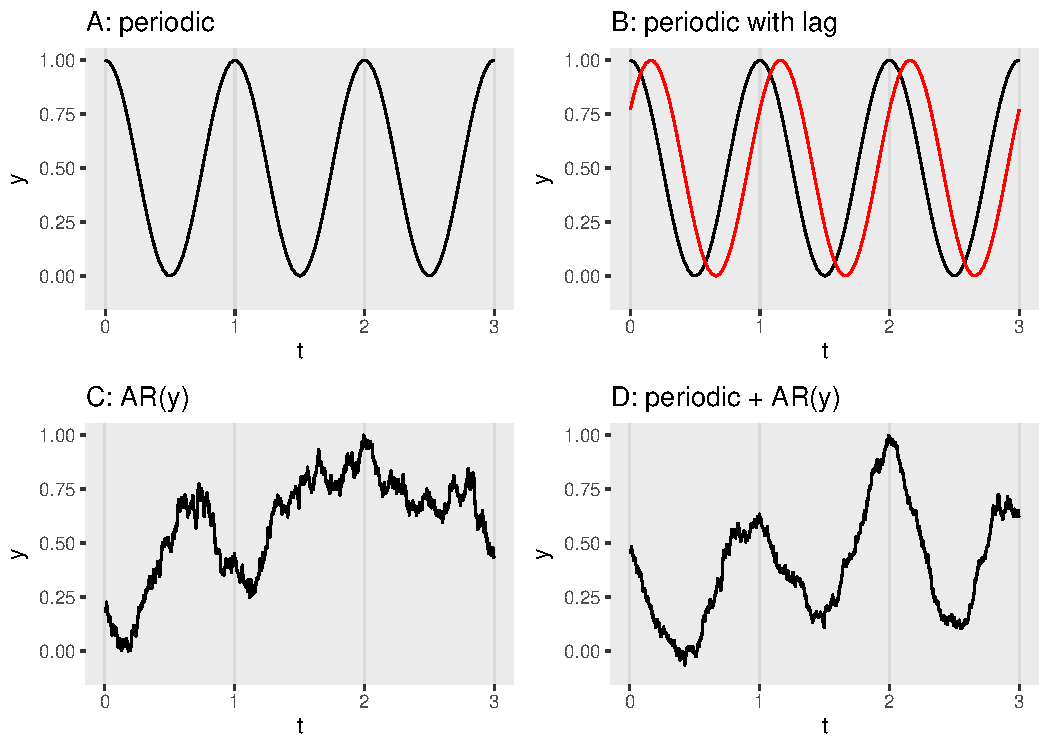
\includegraphics[width=\linewidth]{figures/art_examples.pdf}
\end{frame}

\begin{frame}
  \frametitle{\futureicon\ Planting density and lateral red:far-red ratio}
  \centering
  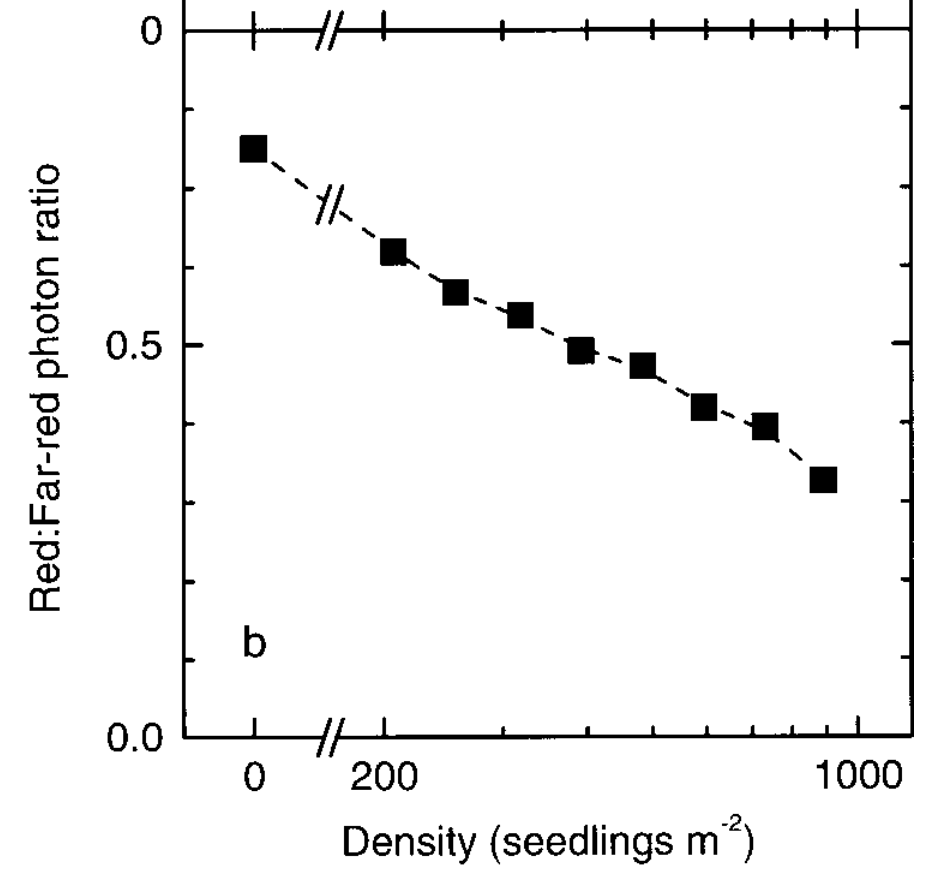
\includegraphics[width=0.66\linewidth]{figures/RFR-density.png}
\end{frame}

\begin{frame}
  \frametitle{\futureicon\ Potential evapotranspiration and UV-B irradiance}
  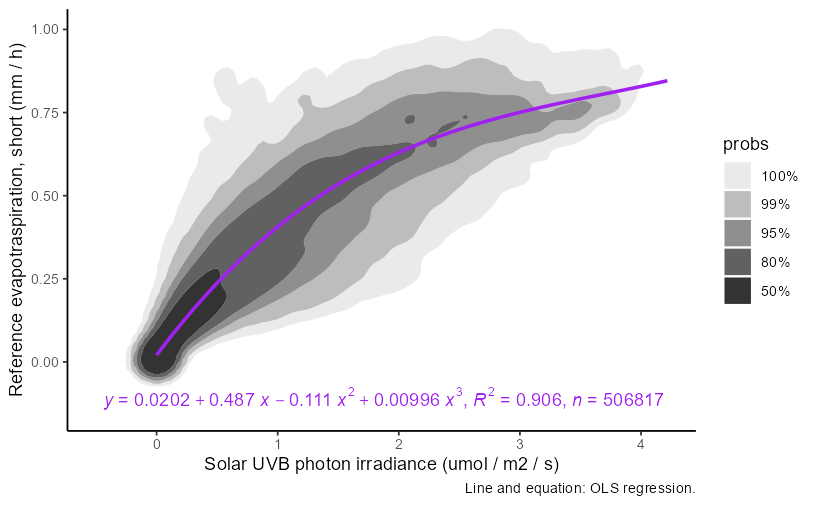
\includegraphics[width=\linewidth]{figures/PET-UVB-2020-2022.png}
\end{frame}

%\begin{frame}
%  \frametitle{Forecasting: its relation to fitness}
%  \begin{itemize}
%    \item I ask you to forget about how information processing is implemented\ldots
%    \item \ldots and consider the idea that every organism must have evolved the capacity to ``forecast'' future events important for its fitness.
%    \item How information is processed, ``the machinery used'', does not need to be the same as long the information is acquired, transmitted, stored and combined successfully.
%  \end{itemize}
%\end{frame}

%\begin{frame}
%\frametitle{Information as a paradigm}
%\begin{enumerate}
%  \item Information and big data are the buzz-words or our time.
%  \item Given us a paradigm that ``asks to be applied''\ldots
%  \item \ldots but care is needed.
%  \item Much like the machine paradigm from the industrial revolution failed to explain life\ldots
%  \item \ldots the use-of-information paradigm will not be enough to explain it.
%  \item However, it is able to explain some aspects of life.
%\end{enumerate}
%\end{frame}

\begin{frame}
\frametitle{\futureicon\ Forecasting and resource investment}
\begin{itemize}
  \item There are reliable and unreliable sources of information.
  \item Forecasting can depend on a single reliable predictor or\ldots
  \item \ldots on a combination of several less reliable predictors.
  \item Predictors \emph{do not need} to have a direct cause-effect relationship.
  \item Forecasts are subject to errors\ldots
  \item \ldots outcomes $\to$ described by probabilities.
  \item Dynamic context $\to$ repeated-tuning of responses.
\end{itemize}
\end{frame}

\begin{frame}{\aclimicon\ Acclimation is a process in time}

{\centering

ENVIRONMENT\\[0.5ex]

{\LARGE\meteosuncloud\hspace{0.9em}\meteosun\hspace{0.9em}\caterpilar\hspace{0.9em}\meteorain\hspace{0.9em}\bug\hspace{0.9em}\Huge\grassplant\hspace{0.9em}}

\resizebox{\linewidth}{!}{%
\footnotesize
  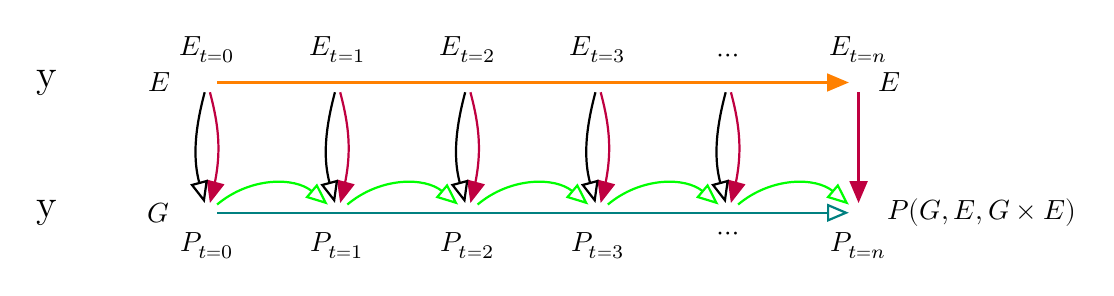
\begin{tikzpicture}[auto]
    \node [aa, label=left:{\Large\timeforwards}] (environment) {};
    \node [aa, below = of environment, label=left:{\Large\timeforwards}] (plant) {};
    \node [aa, right = of environment, label=above:{$E_{t=0}$}, label=left:{$E\ \ $}] (env_zero) {};
    \node [aa, right = of env_zero, label=above:{$E_{t=1}$}] (env_one) {};
    \node [aa, right = of env_one, label=above:{$E_{t=2}$}] (env_two) {};
    \node [aa, right = of env_two, label=above:{$E_{t=3}$}] (env_three) {};
    \node [aa, right = of env_three, label=above:{$\cdots$}] (env_four) {};
    \node [aa, right = of env_four, label=above:{$E_{t=n}$}, label=right:{$E$}] (env_end) {};
    \node [aa, below = of env_zero, label=below:{$P_{t=0}$}, label=left:{$G\ \ $}] (pheno_zero) {};
    \node [aa, below = of env_one, label=below:{$P_{t=1}$}] (pheno_one) {};
    \node [aa, below = of env_two, label=below:{$P_{t=2}$}] (pheno_two) {};
    \node [aa, below = of env_three, label=below:{$P_{t=3}$}] (pheno_three) {};
    \node [aa, below = of env_four, label=below:{$\cdots$}] (pheno_four) {};
    \node [aa, below = of env_end, label=below:{$P_{t=n}$}, label=right:{\ $P(G, E, G \times E)$}] (pheno_end) {};

    \path [llo, below] (env_zero) -- (env_end);
    \path [llt, above] (pheno_zero) -- (pheno_end);

    \path [llr] (env_zero) edge [bend right=-15] (pheno_zero);
    \path [ll] (pheno_zero) edge [bend right=-15] (env_zero);
    \path [llg, above] (pheno_zero) edge [bend right=-40] (pheno_one);

    \path [llr] (env_one) edge [bend right=-15] (pheno_one);
    \path [ll] (pheno_one) edge [bend right=-15] (env_one);
    \path [llg, above] (pheno_one) edge [bend right=-40] (pheno_two);

    \path [llr] (env_two) edge [bend right=-15] (pheno_two);
    \path [ll] (pheno_two) edge [bend right=-15] (env_two);
    \path [llg, above] (pheno_two) edge [bend right=-40] (pheno_three);

    \path [llr] (env_three) edge [bend right=-15] (pheno_three);
    \path [ll] (pheno_three) edge [bend right=-15] (env_three);
    \path [llg, above] (pheno_three) edge [bend right=-40] (pheno_four);

    \path [llr] (env_four) edge [bend right=-15] (pheno_four);
    \path [ll] (pheno_four) edge [bend right=-15] (env_four);
    \path [llg, above] (pheno_four) edge [bend right=-40] (pheno_end);

    \path [llr] (env_end) -- (pheno_end);

  \end{tikzpicture}%
}%

{\LARGE\seedling\hspace{1.9em}\Huge\seedling\hspace{1.5em}\smallplant\hspace{1.5em}\floweringplant}

PLANT\\

}

\end{frame}

\begin{frame}
  \frametitle{\aclimicon\ Acclimation depends on plasticity}
\begin{itemize}
  \item Many responses take time $\Rightarrow$ must be triggered in advance.
  \item Slower responses need to be triggered earlier than faster ones.
  \item Enhanced readiness to respond allows delaying full commitment.
  \item Prediction of future environment is error-prone.
  \item Cost of response is deterministic, benefit is stochastic.
  \item Acclimation is based on syndromes rather than individual responses (?).
\end{itemize}
\end{frame}

%\begin{frame}
%  \frametitle{Vocabulary: information as an abstraction}
%  \begin{itemize}
%    \item Information is encoded in one or more carriers.
%    \item e.g.\ radio broadcasting vs.\ internet-``radio''.
%    \item First a signal (or cue) needs to be sensed or perceived.
%    \item To extract information a signal or cue must be decoded.
%    \item The components of a signal we cannot decode are ``noise''.
%    \item Memory is the storage of information.
%    \item Processing is the combination of different bits of information.
%    \item Communication is the exchange of information between an emitter and a receiver (one-way or two way).
%  \end{itemize}
%\end{frame}
%
\section{\frameicon\ Framework and \planticon\ Plants}

\begin{frame}{\frameicon\ Information-based framework of acclimation}
\onslide<1-2>{\footnotesize
\resizebox{\linewidth}{!}{%
  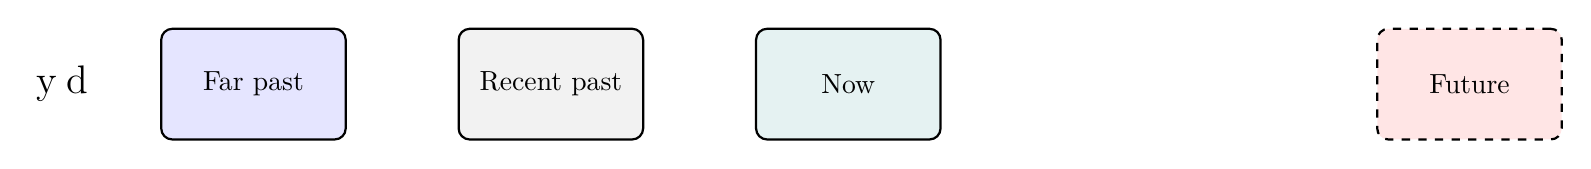
\begin{tikzpicture}[auto]
    \node [a] (environment) {\Large\timeforwards~\timebackwards};
    \node [b, right = of environment, fill=blue!10] (history) {Far past};
    \node [b, right = of history] (recent) {Recent past};
    \node [b, right = of recent, fill=teal!10] (now) {Now};
    \node [d, right = of now, xshift=11.7em] (future) {Future};
\end{tikzpicture}%
}}
\vspace{2em}

\onslide<2-3>{\footnotesize
\resizebox{\linewidth}{!}{%
  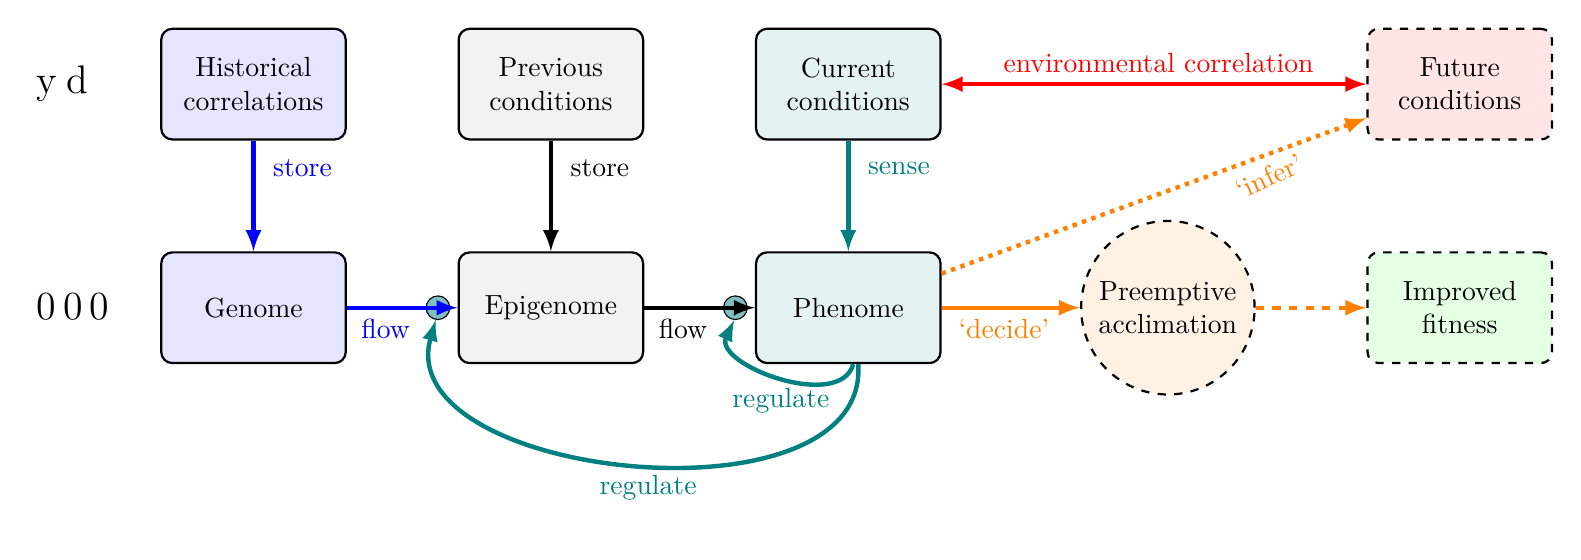
\begin{tikzpicture}[auto]
    \node [a] (environment) {\Large\timeforwards~\timebackwards};
    \node [b, right = of environment, fill=blue!10] (history) {Historical correlations};
    \node [b, right = of history] (stress) {Previous conditions};
    \node [b, right = of stress, fill=teal!10] (data) {Current conditions};
    \node [b, below = of history, fill=blue!10] (genome) {Genome};
    \node [big dot, right = of genome] (valve1) {};
    \node [b, below = of stress] (memory) {Epigenome};
    \node [big dot, right = of memory] (valve2) {};
    \node [b, right = of memory, fill=teal!10] (info) {Phenome};
    \node [a, below = of environment] (plant) {\Large\smallplant\,\smallplant\,\smallplant};
    \node [c, right = of info, fill=orange!10] (acclimation) {Preemptive acclimation};
    \node [d, right = of acclimation, fill=green!10] (ready) {Improved fitness};
    \node [d, above = of ready] (stress2) {Future conditions};

    \path [l] (stress) -- (memory) node[near start,right]{\hspace{0.3em}store};
    \path [lb] (history) -- (genome) node[near start, right]{\hspace{0.3em}store};
    \path [lg] (data) -- (info) node[near start,right]{\hspace{0.3em}sense};
    \path [lb] (genome) -- (memory) node[near start,below]{\hspace{0.8em}flow};
    \path [l] (memory) -- (info) node[near start,below]{\hspace{0.8em}flow};
    \path [lr] (stress2) -- (data) node[near end,above]{\hspace{8em}environmental correlation};
    \path [lo, dotted] (info) -- (stress2) node[near end,below,rotate=25]{`infer'};
    \path [lo] (info) -- (acclimation) node[near start,below]{\hspace{2em}`decide'};
    \path [lo, dashed] (acclimation) -- (ready);
    \path [lg] (info) edge [bend left=100]  node[midway, below]{\hspace{1em}regulate} (valve1);
    \path [lg] (info) edge [bend left=95]  node[midway, below]{regulate\hspace{5em}} (valve2);

\end{tikzpicture}%
}}%
\end{frame}

\begin{frame}{\frameicon\ Preemptive acclimation to shade}
\footnotesize
\resizebox{\linewidth}{!}{%
  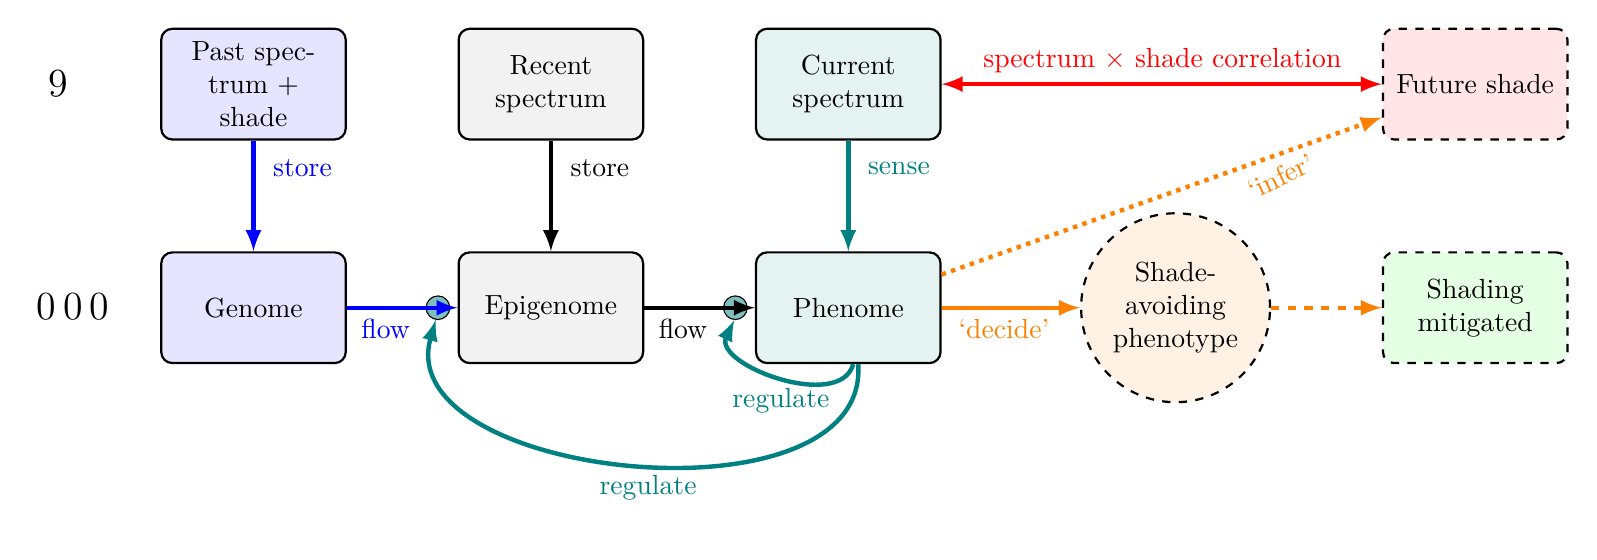
\begin{tikzpicture}[auto]
    \node [a] (environment) {\Large\meteosun\bush};
    \node [b, right = of environment, fill=blue!10] (history) {Past spectrum + shade};
    \node [b, right = of history] (stress) {Recent spectrum};
    \node [b, right = of stress, fill=teal!10] (data) {Current spectrum};
    \node [b, below = of history, fill=blue!10] (genome) {Genome};
    \node [big dot, right = of genome] (valve1) {};
    \node [b, below = of stress] (memory) {Epigenome};
    \node [big dot, right = of memory] (valve2) {};
    \node [b, right = of memory, fill=teal!10] (info) {Phenome};
    \node [a, below = of environment] (plant) {\Large\smallplant\,\smallplant\,\smallplant};
    \node [c, right = of info, fill=orange!10] (acclimation) {Shade-avoiding phenotype};
    \node [d, right = of acclimation, fill=green!10] (ready) {Shading mitigated};
    \node [d, above = of ready] (stress2) {Future shade};

    \path [l] (stress) -- (memory) node[near start,right]{\hspace{0.3em}store};
    \path [lb] (history) -- (genome) node[near start, right]{\hspace{0.3em}store};
    \path [lg] (data) -- (info) node[near start,right]{\hspace{0.3em}sense};
    \path [lb] (genome) -- (memory) node[near start,below]{\hspace{0.8em}flow};
    \path [l] (memory) -- (info) node[near start,below]{\hspace{0.8em}flow};
    \path [lr] (stress2) -- (data) node[near end,above]{\hspace{8em}spectrum $\times$ shade correlation};
    \path [lo, dotted] (info) -- (stress2) node[near end,below,rotate=25]{`infer'};
    \path [lo] (info) -- (acclimation) node[near start,below]{\hspace{2em}`decide'};
    \path [lo, dashed] (acclimation) -- (ready);
    \path [lg] (info) edge [bend left=100]  node[midway, below]{\hspace{1em}regulate} (valve1);
    \path [lg] (info) edge [bend left=95]  node[midway, below]{regulate\hspace{5em}} (valve2);
\end{tikzpicture}%
}%
\end{frame}

\begin{frame}{\frameicon\ Preemptive acclimation to drought}
  \footnotesize
\resizebox{\linewidth}{!}{%
  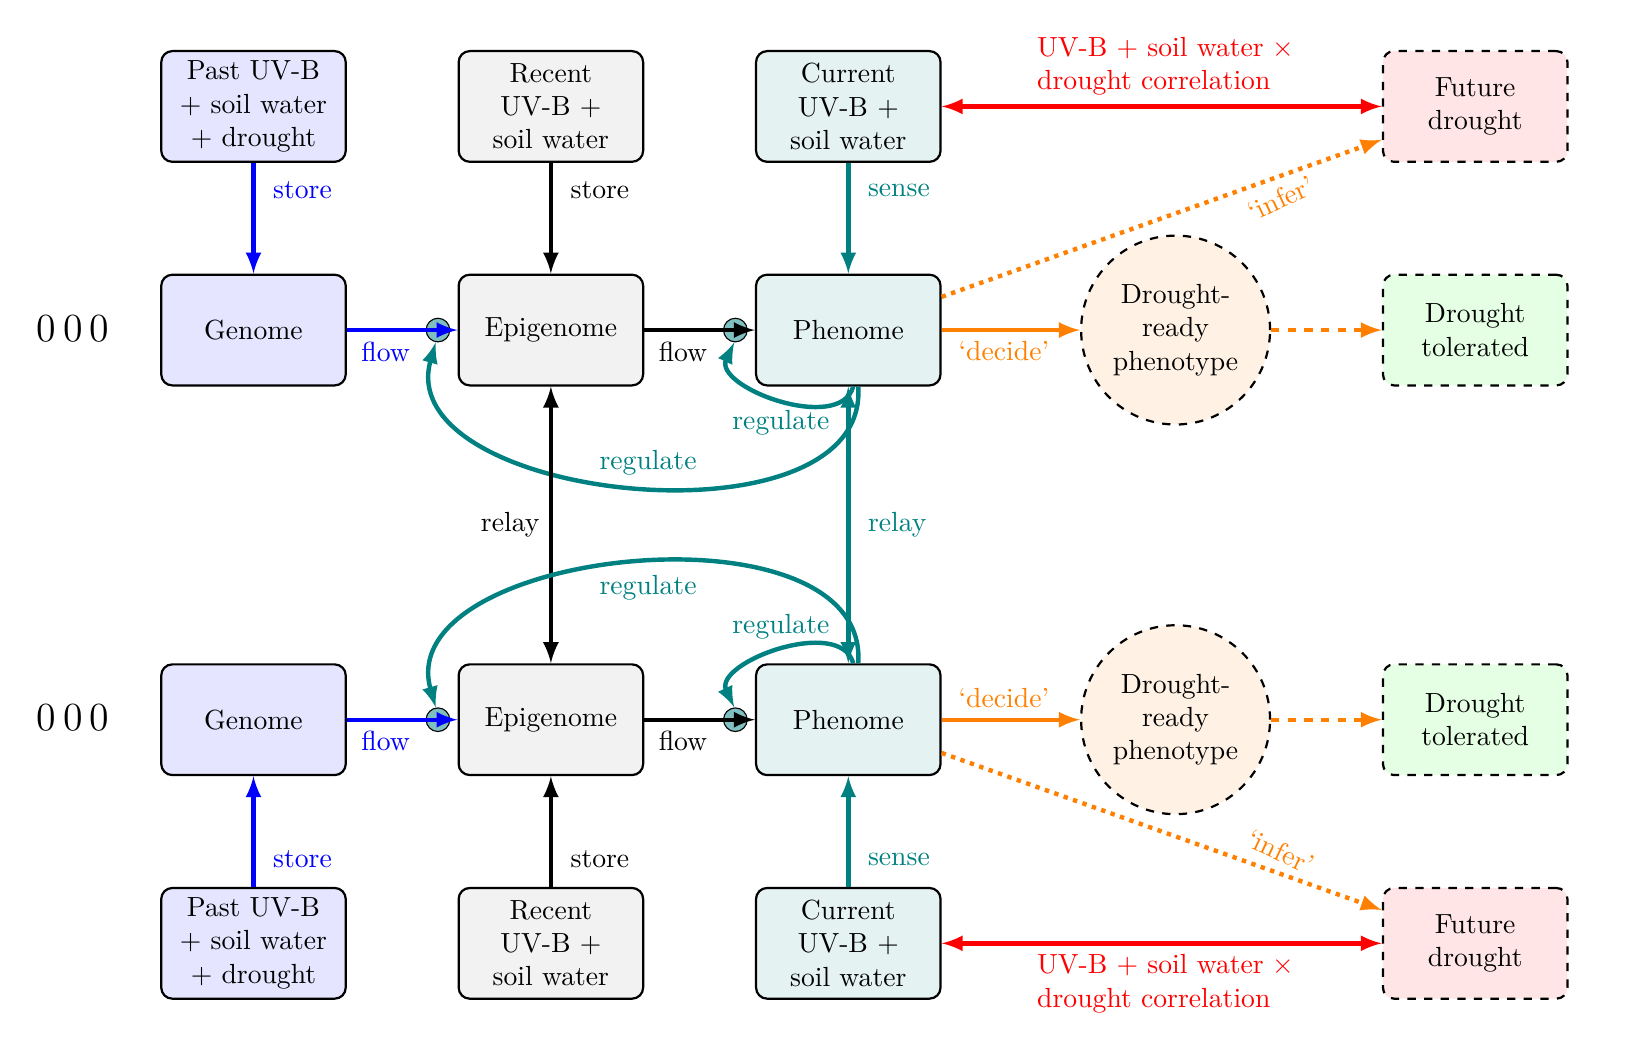
\begin{tikzpicture}[auto]
    \node [a] (environment) {\Large\meteosun\,\meteorain};
    \node [b, right = of environment, fill=blue!10] (history) {Past \mbox{UV-B} + soil water + drought};
    \node [b, right = of history] (stress) {Recent\\ \mbox{UV-B} + soil water};
    \node [b, right = of stress, fill=teal!10] (data) {Current \mbox{UV-B} + soil water};
    \node [b, below = of history, fill=blue!10] (genome) {Genome};
    \node [big dot, right = of genome] (valve1) {};
    \node [b, below = of stress] (memory) {Epigenome};
    \node [big dot, right = of memory] (valve2) {};
    \node [b, right = of memory, fill=teal!10] (info) {Phenome};
    \node [a, below = of environment] (plant) {\Large\smallplant\,\smallplant\,\smallplant};
    \node [c, right = of info, fill=orange!10] (acclimation) {Drought-ready phenotype};
    \node [d, right = of acclimation, fill=green!10] (ready) {Drought tolerated};
    \node [d, above = of ready] (stress2) {Future drought};

    \path [l] (stress) -- (memory) node[near start,right]{\hspace{0.3em}store};
    \path [lb] (history) -- (genome) node[near start, right]{\hspace{0.3em}store};
    \path [lg] (data) -- (info) node[near start,right]{\hspace{0.3em}sense};
    \path [lb] (genome) -- (memory) node[near start,below]{\hspace{0.8em}flow};
    \path [l] (memory) -- (info) node[near start,below]{\hspace{0.8em}flow};
    \path [lr] (stress2) -- (data) node[midway,above]{\hspace{11em}\parbox{20em}{UV-B + soil water $\times$\\ drought correlation}};
    \path [lo, dotted] (info) -- (stress2) node[near end,below,rotate=25]{`infer'};
    \path [lo] (info) -- (acclimation) node[near start,below]{\hspace{2em}`decide'};
    \path [lo, dashed] (acclimation) -- (ready);
    \path [lg] (info) edge [bend left=100]  node[midway, above]{\hspace{1em}regulate} (valve1);
    \path [lg] (info) edge [bend left=95]  node[midway, below]{regulate\hspace{8em}} (valve2);\pause

    \node [b, below = of genome,yshift=-6em, fill=blue!10] (genome1) {Genome};
    \node [big dot, right = of genome1] (valve11) {};
    \node [b, below = of memory,yshift=-6em] (memory1) {Epigenome};
    \node [big dot, right = of memory1] (valve21) {};
    \node [b, right = of memory1, fill=teal!10] (info1) {Phenome};
    \node [a, below = of plant,yshift=-6em] (plant1) {\Large\smallplant\,\smallplant\,\smallplant};
    \node [c, right = of info1, fill=orange!10] (acclimation1) {Drought-ready phenotype};
    \node [d, right = of acclimation1, fill=green!10] (ready1) {Drought tolerated};
    \node [b, below = of info1, fill=teal!10] (data1) {Current \mbox{UV-B} + soil water};
    \node [b, below = of genome1, fill=blue!10] (history1) {Past \mbox{UV-B} + soil water + drought};
    \node [a, left = of history1] (environment1) {\Large\meteosun\,\meteorain};
    \node [b, right = of history1] (stress1) {Recent\\ \mbox{UV-B} + soil water};
    \node [d, below = of ready1] (stress21) {Future drought};

    \path [l] (stress1) -- (memory1) node[near start,right]{\hspace{0.3em}store};
    \path [lb] (genome1) -- (memory1) node[near start,below]{\hspace{0.8em}flow};
    \path [l] (memory1) -- (info1) node[near start,below]{\hspace{0.8em}flow};
    \path [lo, dashed] (acclimation1) -- (ready1);
    \path [lx] (memory) -- (memory1) node[midway,left]{\hspace{0.3em}relay\hspace{0.3em}};
    \path [lgx] (info) -- (info1) node[midway,right]{\hspace{0.3em}relay\hspace{0.3em}};%\pause
    \path [lg] (data1) -- (info1) node[near start,right]{\hspace{0.3em}sense};
    \path [lg] (info1) edge [bend left=-100]  node[midway, below]{\hspace{1em}regulate} (valve11);
    \path [lg] (info1) edge [bend left=-95]  node[midway, above]{regulate\hspace{8em}} (valve21);
    \path [lb] (history1) -- (genome1) node[near start, right]{\hspace{0.3em}store};
    \path [lr] (stress21) -- (data1) node[midway,below]{\hspace{11em}\parbox{20em}{UV-B + soil water $\times$\\ drought correlation}};
    \path [lo, dotted] (info1) -- (stress21) node[near end,above,rotate=-25]{`infer'};
    \path [lo] (info1) -- (acclimation1) node[near start,above]{\hspace{2em}`decide'};

%    \node [b, below = of genome1, fill=blue!10] (genome2) {Genome};
%    \node [big dot, right = of genome2] (valve12) {};
%    \node [b, below = of memory1] (memory2) {Epigenome};
%    \node [big dot, right = of memory2] (valve22) {};
%    \node [b, right = of memory2, fill=teal!10] (info2) {Phenome};
%    \node [a, below = of plant1] (plant2) {\Large\smallplant\,\smallplant\,\smallplant};
%    \node [c, right = of info2, fill=orange!10] (acclimation2) {Drought-ready phenotype};
%    \node [d, right = of acclimation2, fill=green!10] (ready2) {Drought tolerated};
%
%    \path [lb] (genome2) -- (memory2) node[near start,below]{\hspace{0.8em}flow};
%    \path [l] (memory2) -- (info2) node[near start,below]{\hspace{0.8em}flow};
%    \path [lo] (info2) -- (acclimation2) node[near start,below]{\hspace{2em}`decide'};
%    \path [lo, dashed] (acclimation2) -- (ready2);
%    \path [l] (memory1) -- (memory2) node[near start,right]{\hspace{0.3em}relay};
%    \path [lg, dashed] (info1) -- (info2) node[near start,right]{\hspace{0.3em}relay};


\end{tikzpicture}%
}%
\end{frame}

\begin{frame}
\frametitle{\planticon\ Data processing mechanism in plants I}
\begin{itemize}
  \item We know something on how decoding works\ldots
  \item \ldots for some individual cues or signals.
  \item A frequent \emph{naive model} is a linear chain of events.
  \item Cue/signal perception $\rightarrow$ direct decoding of information $\rightarrow$ response
  \item Low R:FR $\rightarrow$ ``means shade'' $\rightarrow$ shade avoidance response
  \item Can frequently describe responses to single cues or signals
\end{itemize}
\end{frame}

\begin{frame}
\frametitle{\planticon\ Data processing mechanism in plants II}
\begin{itemize}
  \item We know almost nothing on how decoding works\ldots
  \item[] \ldots for sets of cues or signals.
  \item A complex and realistic (?) model is a network of interactions, memories and feedback loops.
  \item Synchronous and asynchronous perception of cues/signals $\rightarrow$ \ldots
  \item[] complex decoding of information $\rightarrow$\ldots
    adjustment of ready-ness to respond.
  \item Synchronous and asynchronous perception of cues/signals $\rightarrow$ \ldots
  \item[] complex decoding of information + readiness state $\rightarrow$ response.
\end{itemize}
\end{frame}

\section{\shopbagicon\ Take Home Message}

\begin{frame}
  \frametitle{\shopbagicon\ Temporal and spatial context matters}
  \begin{enumerate}
    \item Components of signalling networks can be best teased out in unnatural contexts including single factor experiments.
    \item Regulation and signalling interactions can be meaningfully described only in real or realistic contexts preferably using factorial experiments.
    \item Describing a syndrome requires in most cases parallel measurements at different levels of organization.
    \item Time courses of response and responsiveness need to be followed.
    \item Neighbours communicate and share information and miss-information.
  \end{enumerate}
\end{frame}

\begin{frame}[fragile,allowframebreaks]
  \frametitle{References}
  \nocite{Falik2022,Falik2023,Novoplansky2016a,Robson2014,Sadras2021,Sadras2021,Sadras2021,Aphalo1995}
{\renewcommand{\bibopenparen}{\adddot\addspace}
\renewcommand{\bibcloseparen}{\adddot\addspace}
\begin{refcontext}[sorting=nyt]
\renewrobustcmd*{\revsdnamepunct}{}
\renewrobustcmd*{\mkbibnamefamily}[1]{\textbf{#1}}
\renewrobustcmd*{\mkbibnamegiven}[1]{\textbf{#1}}
\printbibliography
\end{refcontext}}
\end{frame}

\end{document}

	\begin{frame}[c]
		\begin{center}
			\begin{small}
				\copyright 2016--2020 by Pedro J. Aphalo\\
				Organismal and Evolutionary Biology Research Programme, University of Helsinki, Finland.\\
				\textcolor{blue}{\url{http://blogs.helsinki.fi/senpep-blog/}}\\[2ex]
			\end{small}

			\begin{footnotesize}
				`The evolutionary ecology of information acquisition in plants' slides from a presentation by Pedro J. Aphalo are licensed under a Creative Commons Attribution-ShareAlike 4.0 International License.\\[2ex]

			\end{footnotesize}

			
\includegraphics[width=6em]{figures/by-sa}
		\end{center}
	\end{frame}


\begin{frame}
\frametitle{Listener perspective}
\begin{enumerate}
  \item Contribution to own fitness
  \item Own response
  \item Decoding of information
  \item Perception
  \item Available cues/signals
\end{enumerate}
\end{frame}

\begin{frame}
\frametitle{Emitter perspective}
\begin{enumerate}
  \item Contribution to own fitness
  \item Response from listener
  \item Encoding of information
  \item Emission
  \item Broadcasted signals
\end{enumerate}
\end{frame}

\begin{frame}
  \frametitle{Data analysis and interpretation}
  \begin{itemize}
    \item Search for patterns of response across mutants and treatments/conditions.
    \item Be careful about quality of gene annotations.
    \item Be very careful about gene ontology (GO) terms.
    \item With PCR have enough reference genes.
  \end{itemize}
\end{frame}

